\chapter{Evaluation}
\label{sec:evaluation}

We evaluate our contributions on an English and a German datasets of comments datasets: YNACC and OMPC.
The datasets were introduced in Section~\ref{ch:datasets}.

\section{Experiments on Yahoo News Annotated Comments Corpus}

The Yahoo News Comment Corpus (YNACC) was intensively presented in Section~\ref{sec:datasets_ynacc}. We compare across three different approaches: baselines, conversation-agnostic models, and our conversation-aware models. 
\subsection{Setup}

For all experiments, we follow the dataset's preprocessing steps of the related work that reported values on YNACC~\cite{napoles2017finding}.
These were presented in Section~\ref{subsec:datasets_ynacc_description}.
Since there are already published results on this dataset, it sets our contribution into perspective.
We train a model for each category separately, as done by the related work.
The experiments and their results are managed via Sacred\footnote{\url{https://github.com/IDSIA/sacred}}.
The setup is different for each method so we describe them in detail in the following.

\subsubsection{Baselines}

We use three different methods as baseline: Naive Bayes, Ridge Regression and the FastText classifier.
All of them are linear classifiers.
The first two are traditional machine learning methods and the follow the bag-of-words idea.
The FastText classifier also considers N-gram of words.
It was introduced by Joulin et al.~\cite{E17-2068} and it outperforms even neural models while being up to $35.000$ times faster.
In addition to the data cleaning described in Section~\ref{subsec:ynacc_data_cleaning}, the tokens are lower-cased.
The default tokenizer of the respective implementation is used. For Naive Bayes and Ridge Regression, we use the Python package \textit{Scikit-Learn}\footnote{\url{https://scikit-learn.org}} in version 0.20.2. For Naive Bayes, we use \textit{MultinomialNB} with the default parameters. For Ridge Regression, we use the cross validation variant on the training data with, as well, the default parameters. For FastText, we use the Python wrapper of the official implementation\footnote{\url{https://github.com/facebookresearch/fastText/tree/master/python}}, version 0.2.0. Because the time to train is short, we use a random search for $1000$ times over the following uniformly distributed hyper-parameters: learning rate from 0 to 1, number of epochs from 5 to 50, N-grams for n from 1 to 5, minimum count for each token from 1 to 10.

\subsubsection{Conversation-agnostic Neural Models}
\label{ssssss:whaaatever}

We use two different language-model-based approaches as comparison models: ULMFIT and BERT. BERT is more advanced than ULMFIT, but it also requires more computation. Because of our financial constraints, we choose ULMFIT as the main reference model. For ULMFIT, we use the author's accompanied implementation in the FastAI library\footnote{\url{https://github.com/fastai/fastai}} in version 1.0.41. ULMFIT internally uses the SpaCy library\footnote{\url{https://spacy.io}} version 2.0 to tokenize the text. We as well clean our data as described in Section~\ref{subsec:ynacc_data_cleaning}. We choose a vocabulary size of $30k$ since it covers over $98.2\%$ of the tokens as shown in Figure~\ref{fig:word_based_anal}.
The use all special text preprocessing steps of the default FastAI implementation.
These are: tokens are lower cased, but for every uppercase word a special uppercase token is prepended. The same applies for all capitalized tokens. In addition, repeating tokens are replaced by a single token and the number of how often it was repeated gets prepended. For instance, ``yes !!!!!'' is transformed to ``yes xxrep 5 !''.

Before training the classifier, the pre-trained WikiText 103 language model needs to get fine-tuned. We choose the datasets of unlabeled comments together with the labeled training comments we noted as YC\textsubscript{LM} in Section~\ref{subsec:datasets_ynacc_description}. Characteristics of the datasets were presented in the section exhaustively. So we fine-tune the language model until overfitting. Even though the authors suggest to fine-tune cautiously, the number of unlabeled samples should be enough (about 200k).
We use random search over the following parameters: epochs 2 to 6, dropout factor from 0.8 to 1.1.
The learning rate scheduler is used to determine a learning rate.
There are 5 different kind of dropout in the model and the authors suggest to tune a specific dropout multiplier.
 And the layer factor, which sets different learning rate for each layer, is set to 2.6.
The authors obtained the magic numbers for the parameters with grid search and they recommend to follow them.
We only save the model with the best validation loss.
The validation set consists of the last $10\%$ of the discussion IDs.

For fine-tuning the classifier, we made the experience that results with the one cycle policy scheduling are unstable. The scheduler is suggested by the authors of the ULMFIT paper. The results varied a lot for different runs with the same parameters. This made it hard to compare the results and thus we abandon it. We use the standard Adam optimizer~\cite{kingma:adam} with the weight decay fix~\cite{loshchilov2017decoupled}.
We used a dropout multiplier of 0.6, 0.7 and 0.8 and a batch size of 64.
The learning rate is set to 0.001, since the learning rate finder did not yield useful results.
The maximum number of epochs is 200 but the learning is stopped, when the Cohen's Kappa score does not improve for 10 epochs (``early stopping''). Only the model with the best Cohen's Kappa score is saved. 

BERT by Devlin et al.~\cite{devlin2018bert} was already briefly mentioned in Section~\ref{sec:bgrd_tlwlm}. While we focus on ULMFIT in this work, the approach of BERT is similar. It requires more computation which is the reason we cannot use it for all our experiments. It is not feasible for us to fine-tune the language model on our domain of news comments. Thus, we use only a pre-trained BERT model. Out of familiarity with PyTorch, we use the port to PyTorch\footnote{\url{https://github.com/huggingface/pytorch-pretrained-BERT}}, which replicated the results of the original TensorFlow implementation. We chose the smaller English \textit{Bert Cased} model because we hypothesize that the casing in comments bears information. The approach operates on sub-word basis and did not require any preprocessing. First, we manually explored a range of useful hyper-parameters and then did a grid search over them. The parameters were: number of epochs from 3 to 10, the learning $5e^{-6}$, $5e^{-7}$, $5e^{-8}$.

\subsubsection{Prepend Previous}

For computational reason, we only evaluate Prepend Previous on the ULMFIT language model approach. The setup is the same as described for conversation-agnostic model in the previous section. Only the dropout multipliers are modified to 0.9, 1, 1.1, 1.2, 1.3. Comments are cut to 200, the total maximum token length is 1400 to optimize RAM usage. The learning rate is set to 0.001 and batch size to 64. Maximum number of epochs is 200 and early stopping is used.
The samples were truncated in the beginning. There are five different variations of Prepend Previous:

\begin{table}[H]
\caption{Variations of Prepend Previous}
\label{tab:eval_ynacc_setup}
\begin{tabular}{l l}
\toprule
Variation & Description \\
\midrule
TX\textsubscript{1} & text \\
TX\textsubscript{2} & text, the language model is not fine-tuned  \\
 HL\textsubscript{1} & text, headline is prepended to all top-level comments all the time \\
 HL\textsubscript{2} & text, headline is only prepended to top-level comments if they would be alone \\
 ART & text, headline, article (if available) \\
\bottomrule
\end{tabular}	
\end{table}

The difference between TX\textsubscript{1} and TX\textsubscript{2} is whether the fine-tuning of the language model has to be done on preprocessed comments (TX\textsubscript{1}) or on non-preprocessed comments (TX\textsubscript{2}). The language model for TX\textsubscript{2} was identical to the conversation-agnostic comparison models. For HL\textsubscript{1}, information about the article are always included. For HL\textsubscript{2}, the information was only included for top-level comments.
Since we do not have all articles, we cannot add all the articles for ART.

\subsection{Results}
\label{sec:exp_ynacc_results}

As metrics, we use F\textsubscript{1 micro}, which is equivalent to accuracy in this setup, F\textsubscript{1 macro} and, Cohen's Kappa (or short Kappa).
We explained Kappa in Section~\ref{sec:metrics} and gives a meaningful value even on unbalanced categories.
The full results including the test values are in Appendix~\ref{ch:ynacc_full}.
We only focus on validation results, since the related work does not report test results.
In addition, the test results differ greatly from the validation results across all models -- baselines as well as neural models.
For instance, Kappa increased in the category Audience by about 0.1 points for almost all models.
Also a simple ridge regression pushes the Kappa score from 0.52 to 0.66.
Even though the ridge regression baseline generally achieves poor results.
For all other categories, the performance deteriorates drastically on the test dataset.
For Off-topic, the differences are the most significant.
While on the validation sets, the Kappa score drops to below 0.2 for all models while performing on the validation set up to 0.48.
The further implications of these results will be discussed later.

In Table~\ref{tab:res1} are the results of the baseline compared to conversation-agnostic models.
The left side of the table consists of the comment's text only.
The right side of the text and a binary feature of whether a comment is a top-level comment or a reply.
This feature greatly improves the performance for the category Audience for all models.
However, for Agreement, Informative, Controversial and Off-topic the results decrease.
For the remaining categories are the differences negligible. In general, the FastText classifier outperformed the other baselines by far.
On the comment's text and reply, it achieved the best results on Audience by a margin of 0.04 F\textsubscript{1 micro} score.
BERT is overall the winner even though the language model was not fine-tuned on comments.
For Controversial, it outperforms other approaches by a margin of about 0.05 F\textsubscript{1 micro} score.
ULMFIT achieves slightly worse performance than BERT but still outperforms the baselines on the vast majority of categories.

\begin{table}
\small
\caption{Experiment results of baselines and conversation-agnostic comparison models on the YNACC validation dataset. The highst value for each row is highlighted. Since BERT~(BT) is out of competition, its values are underlined if it would have achieved the highest results. Naive Bayes~(NB), Ridge Regression~(RR), FastText Classifier~(FT), ULMFIT~(UF).}
\begin{tabular}{ l l l l l l l l l l l l}
\toprule
\multicolumn{2}{l}{} & \multicolumn{5}{c}{Text} & \multicolumn{5}{c}{Text + Reply} \\
\cmidrule(r){3-7}
\cmidrule(r){8-12}
Category & Metric &  NB & RR & FT & UF & BT & NB & RR & FT & UF & BT\\
\midrule
\addlinespace[2ex]
\multirow{3}{*}{Persuasive} & F\textsubscript{1 micro} & 0.814 & 0.855 & 0.871 & 0.845 & 0.864 & 0.835 & \textbf{0.876} & 0.874 & 0.830 & 0.862 \\
& F\textsubscript{1 macro} & 0.544 & 0.645 & 0.681 & 0.634 & \underline{0.721} & 0.578 & 0.655 & \textbf{0.694} & 0.684 & \underline{0.721} \\
& Kappa & 0.097 & 0.298 & 0.369 & 0.273 & 0.442 & 0.168 & 0.326 & \textbf{0.393} & 0.370 & \underline{0.443} \\ \addlinespace[2ex]
\multirow{3}{*}{Audience} & F\textsubscript{1 micro} & 0.686 & 0.698 & 0.741 & 0.746 & 0.795 & 0.783 & 0.809 & \textbf{0.876} & 0.834 & 0.831 \\
& F\textsubscript{1 macro} & 0.586 & 0.594 & 0.677 & 0.708 & 0.765 & 0.728 & 0.753 & \textbf{0.829} & 0.790 & 0.803 \\
& Kappa & 0.207 & 0.228 & 0.369 & 0.417 & 0.532 & 0.470 & 0.524 & \textbf{0.662} & 0.591 & 0.608 \\ \addlinespace[2ex]
\multirow{3}{*}{Agreement} & F\textsubscript{1 micro} & 0.885 & 0.879 & 0.902 & 0.907 & 0.903 & 0.885 & 0.885 & 0.905 & \textbf{0.912} & 0.903 \\
& F\textsubscript{1 macro} & 0.497 & 0.494 & 0.673 & \textbf{0.719} & 0.709 & 0.497 & 0.555 & 0.672 & 0.696 & \underline{0.727} \\
& Kappa & 0.046 & 0.035 & 0.357 & \textbf{0.444} & 0.423 & 0.046 & 0.140 & 0.357 & 0.404 & \underline{0.457} \\ \addlinespace[2ex]
\multirow{3}{*}{Informat.} & F\textsubscript{1 micro} & 0.818 & 0.818 & 0.816 & \textbf{0.866} & 0.862 & 0.826 & 0.821 & 0.821 & 0.847 & 0.845 \\
& F\textsubscript{1 macro} & 0.558 & 0.528 & 0.614 & \textbf{0.683} & \underline{0.748} & 0.553 & 0.494 & 0.623 & 0.679 & 0.717 \\
& Kappa & 0.136 & 0.087 & 0.233 & \textbf{0.378} & \underline{0.496} & 0.135 & 0.037 & 0.251 & 0.362 & 0.434 \\ \addlinespace[2ex]
\multirow{3}{*}{Mean} & F\textsubscript{1 micro} & 0.813 & 0.813 & 0.826 & \textbf{0.842} & \underline{0.849} & 0.811 & 0.813 & 0.823 & 0.840 & 0.835 \\
& F\textsubscript{1 macro} & 0.640 & 0.630 & 0.666 & 0.726 & 0.740 & 0.641 & 0.619 & 0.674 & \textbf{0.752} & 0.723 \\
& Kappa & 0.296 & 0.280 & 0.348 & 0.457 & 0.484 & 0.297 & 0.263 & 0.359 & \textbf{0.504} & 0.448 \\ \addlinespace[2ex]
\multirow{3}{*}{Controv.} & F\textsubscript{1 micro} & 0.663 & 0.641 & 0.687 & \textbf{0.706} & 0.735 & 0.691 & 0.703 & 0.704 & \textbf{0.706} & \underline{0.758} \\
& F\textsubscript{1 macro} & 0.639 & 0.574 & 0.644 & \textbf{0.675} & 0.700 & 0.661 & 0.590 & 0.663 & 0.672 & \underline{0.722} \\
& Kappa & 0.286 & 0.149 & 0.289 & \textbf{0.353} & 0.400 & 0.325 & 0.212 & 0.326 & 0.346 & \underline{0.445} \\ \addlinespace[2ex]
\multirow{3}{*}{Disagree.} & F\textsubscript{1 micro} & 0.634 & 0.646 & 0.703 & 0.756 & 0.739 & 0.660 & 0.701 & 0.737 & \textbf{0.778} & 0.777 \\
& F\textsubscript{1 macro} & 0.626 & 0.639 & 0.682 & 0.745 & 0.729 & 0.654 & 0.687 & 0.724 & \textbf{0.772} & 0.770 \\
& Kappa & 0.254 & 0.280 & 0.368 & 0.491 & 0.459 & 0.312 & 0.375 & 0.448 & \textbf{0.546} & 0.540 \\ \addlinespace[2ex]
\multirow{3}{*}{Off-topic} & F\textsubscript{1 micro} & 0.682 & 0.663 & 0.687 & \textbf{0.749} & 0.737 & 0.704 & 0.668 & 0.680 & 0.706 & 0.740 \\
& F\textsubscript{1 macro} & 0.543 & 0.539 & 0.608 & \textbf{0.670} & 0.663 & 0.601 & 0.625 & 0.609 & 0.644 & \underline{0.676} \\
& Kappa & 0.127 & 0.105 & 0.222 & \textbf{0.353} & 0.334 & 0.222 & 0.252 & 0.222 & 0.290 & \underline{0.357} \\ \addlinespace[2ex]
\multirow{3}{*}{Sentiment} & F\textsubscript{1 micro} & 0.548 & 0.533 & 0.564 & 0.622 & 0.633 & 0.554 & 0.536 & 0.577 & \textbf{0.628} & \underline{0.638} \\
& F\textsubscript{1 macro} & 0.248 & 0.290 & 0.381 & 0.417 & \underline{0.471} & 0.256 & 0.303 & 0.358 & \textbf{0.448} & 0.450 \\
& Kappa & 0.099 & 0.102 & 0.228 & 0.315 & \underline{0.377} & 0.107 & 0.133 & 0.232 & \textbf{0.322} & 0.374 \\ \addlinespace[2ex]
\midrule
\addlinespace[2ex]
\multirow{3}{*}{Average}  & F\textsubscript{1 micro} & 0.727 & 0.727 & 0.755 & 0.782 & 0.790 & 0.749 & 0.756 & 0.777 & \textbf{0.786} & \underline{0.798} \\ & F\textsubscript{1 macro} & 0.542 & 0.548 & 0.625 & 0.664 & 0.694 & 0.574 & 0.586 & 0.649 & \textbf{0.681} & \underline{0.701} \\ & Kappa & 0.172 & 0.173 & 0.309 & 0.386 & 0.438 & 0.231 & 0.251 & 0.361 & \textbf{0.415} & \underline{0.456} \\ \addlinespace[2ex]
\bottomrule
\end{tabular}
\label{tab:res1}
\end{table}

\begin{table}
%\small
\caption{Experiment results on the YNACC validation dataset comparing conversation-agnostic models with conversation-aware models. The former group of models stems from Table~\ref{tab:res1}. The latter were explained in Table~\ref{tab:eval_ynacc_setup}. The highest value in each row is highlighted.}
\begin{tabular}{ l l l l l l l l l l}
\toprule
\multicolumn{2}{l}{} & \multicolumn{3}{c}{Conversation-agnostic} & \multicolumn{5}{c}{Conversation-aware} \\
\cmidrule(r){3-5}
\cmidrule(r){6-10}
Category & Metric & UF\textsubscript{text} & FT\textsubscript{reply} & UF\textsubscript{reply} & TX\textsubscript{1} & TX\textsubscript{2} & HL\textsubscript{1} & HL\textsubscript{2} & ART\\
\midrule
\addlinespace[2ex]
\multirow{3}{*}{Persuasive} & F\textsubscript{1 micro} & 0.845 & \textbf{0.874} & 0.830 & 0.847 & 0.845 & 0.847 & 0.871 & 0.811 \\
& F\textsubscript{1 macro} & 0.634 & 0.694 & 0.684 & 0.703 & 0.674 & 0.688 & \textbf{0.720} & 0.651 \\
& Kappa & 0.273 & 0.393 & 0.370 & 0.407 & 0.348 & 0.378 & \textbf{0.442} & 0.303 \\ \addlinespace[2ex]
\multirow{3}{*}{Audience} & F\textsubscript{1 micro} & 0.746 & \textbf{0.876} & 0.834 & 0.836 & 0.827 & 0.839 & 0.826 & 0.833 \\
& F\textsubscript{1 macro} & 0.708 & \textbf{0.829} & 0.790 & 0.796 & 0.777 & 0.794 & 0.797 & 0.785 \\
& Kappa & 0.417 & \textbf{0.662} & 0.591 & 0.600 & 0.569 & 0.600 & 0.596 & 0.583 \\ \addlinespace[2ex]
\multirow{3}{*}{Agreement} & F\textsubscript{1 micro} & 0.907 & 0.905 & 0.912 & \textbf{0.921} & 0.912 & \textbf{0.921} & 0.915 & 0.909 \\
& F\textsubscript{1 macro} & 0.719 & 0.672 & 0.696 & 0.761 & 0.746 & 0.761 & \textbf{0.763} & 0.731 \\
& Kappa & 0.444 & 0.357 & 0.404 & 0.526 & 0.494 & 0.526 & \textbf{0.529} & 0.466 \\ \addlinespace[2ex]
\multirow{3}{*}{Informative} & F\textsubscript{1 micro} & \textbf{0.866} & 0.821 & 0.847 & 0.847 & 0.843 & 0.859 & 0.845 & 0.826 \\
& F\textsubscript{1 macro} & 0.683 & 0.623 & 0.679 & \textbf{0.695} & 0.672 & 0.693 & 0.690 & 0.666 \\
& Kappa & 0.378 & 0.251 & 0.362 & 0.391 & 0.348 & \textbf{0.392} & 0.381 & 0.334 \\ \addlinespace[2ex]
\multirow{3}{*}{Mean} & F\textsubscript{1 micro} & 0.842 & 0.823 & 0.840 & 0.814 & 0.840 & \textbf{0.845} & 0.838 & 0.826 \\
& F\textsubscript{1 macro} & 0.726 & 0.674 & \textbf{0.752} & 0.726 & 0.724 & 0.749 & 0.738 & 0.727 \\
& Kappa & 0.457 & 0.359 & \textbf{0.504} & 0.453 & 0.453 & 0.500 & 0.477 & 0.455 \\ \addlinespace[2ex]
\multirow{3}{*}{Controversial} & F\textsubscript{1 micro} & 0.706 & 0.704 & 0.706 & 0.728 & 0.725 & 0.727 & 0.728 & \textbf{0.739} \\
& F\textsubscript{1 macro} & 0.675 & 0.663 & 0.672 & 0.679 & 0.672 & 0.684 & 0.686 & \textbf{0.689} \\
& Kappa & 0.353 & 0.326 & 0.346 & 0.360 & 0.346 & 0.369 & 0.372 & \textbf{0.380} \\ \addlinespace[2ex]
\multirow{3}{*}{Disagreement} & F\textsubscript{1 micro} & 0.756 & 0.737 & 0.778 & \textbf{0.794} & 0.782 & 0.792 & 0.785 & 0.763 \\
& F\textsubscript{1 macro} & 0.745 & 0.724 & 0.772 & \textbf{0.786} & 0.773 & 0.783 & 0.777 & 0.756 \\
& Kappa & 0.491 & 0.448 & 0.546 & \textbf{0.572} & 0.547 & 0.567 & 0.554 & 0.513 \\ \addlinespace[2ex]
\multirow{3}{*}{Off-topic} & F\textsubscript{1 micro} & 0.749 & 0.680 & 0.706 & 0.754 & 0.763 & 0.758 & \textbf{0.770} & 0.753 \\
& F\textsubscript{1 macro} & 0.670 & 0.609 & 0.644 & 0.722 & 0.712 & 0.702 & \textbf{0.740} & 0.711 \\
& Kappa & 0.353 & 0.222 & 0.290 & 0.444 & 0.426 & 0.407 & \textbf{0.481} & 0.423 \\ \addlinespace[2ex]
\multirow{3}{*}{Sentiment} & F\textsubscript{1 micro} & 0.622 & 0.577 & 0.628 & \textbf{0.647} & 0.615 & 0.603 & 0.610 & 0.608 \\
& F\textsubscript{1 macro} & 0.417 & 0.358 & \textbf{0.448} & 0.408 & 0.420 & 0.409 & 0.411 & 0.421 \\
& Kappa & 0.315 & 0.232 & 0.322 & \textbf{0.361} & 0.321 & 0.318 & 0.328 & 0.324 \\ \addlinespace[2ex]
\midrule
\addlinespace[2ex]
\multirow{3}{*}{Average}  & F\textsubscript{1 micro} & 0.782 & 0.777 & 0.786 & \textbf{0.798} & 0.794 & \textbf{0.798} & \textbf{0.798} & 0.785 \\ & F\textsubscript{1 macro} & 0.664 & 0.649 & 0.681 & 0.697 & 0.685 & 0.695 & \textbf{0.702} & 0.681 \\ & Kappa & 0.386 & 0.361 & 0.415 & 0.457 & 0.428 & 0.450 & \textbf{0.462} & 0.420 \\ \addlinespace[2ex]
\bottomrule
\end{tabular}
\label{tab:res2}
\end{table}


In Table~\ref{tab:res2} are the results of conversation-aware model in comparison to three best-scoring conversation-agnostic models from Table~\ref{tab:res1}.
On average, context-aware models achieve superior results.
The F\textsubscript{1 micro}, F\textsubscript{1 micro} and Kappa scores increased by 1.53\%, 3.08\% and 11.33\%, respectivly.
Off-topic is the greatest beneficiary with an increase by 36.26\% in Kappa score.
The change in percent is visualized in Figure~\ref{fig:res_changes}.
However, there are differences among the categories.
For Audience and Mean, the performance decreased.
For others such as Agreement, Disagreement, Controversial and Off-topic all metrics improved.
We tested several variations of Prepend Previous.
The first question was whether it is important to fine-tune the language model with preprocessed tokens.
TX\textsubscript{1} outperforms TX\textsubscript{2} in almost all metrics for all categories.
Then, it seems that adding more information does not always seem to help.
Especially, adding information about the article does in some cases decrease the results.
The results of HL\textsubscript{1} and HL\textsubscript{2} differ only slightly.
Only for Persuasive and Off-Topic HL\textsubscript{2} outperforms clearly.
Adding even more information, such as the whole article text, seem to decrease the performance almost all categories.
Only Controversial achieved the best results for ART.
In order to understand the differences for the conversation-aware models, we investigate the effect of it at the example of the category Off-topic.
The conversation-aware model outperform conversation-agnostic models especially when the comments is short. For longer comments, the performance decreased. This is visualized in Figure~\ref{fig:exp_acc_len}. The overall performance increased since the majority of the comments is short (Figure~\ref{fig:len_com}).

\begin{figure}
  \begin{center}
    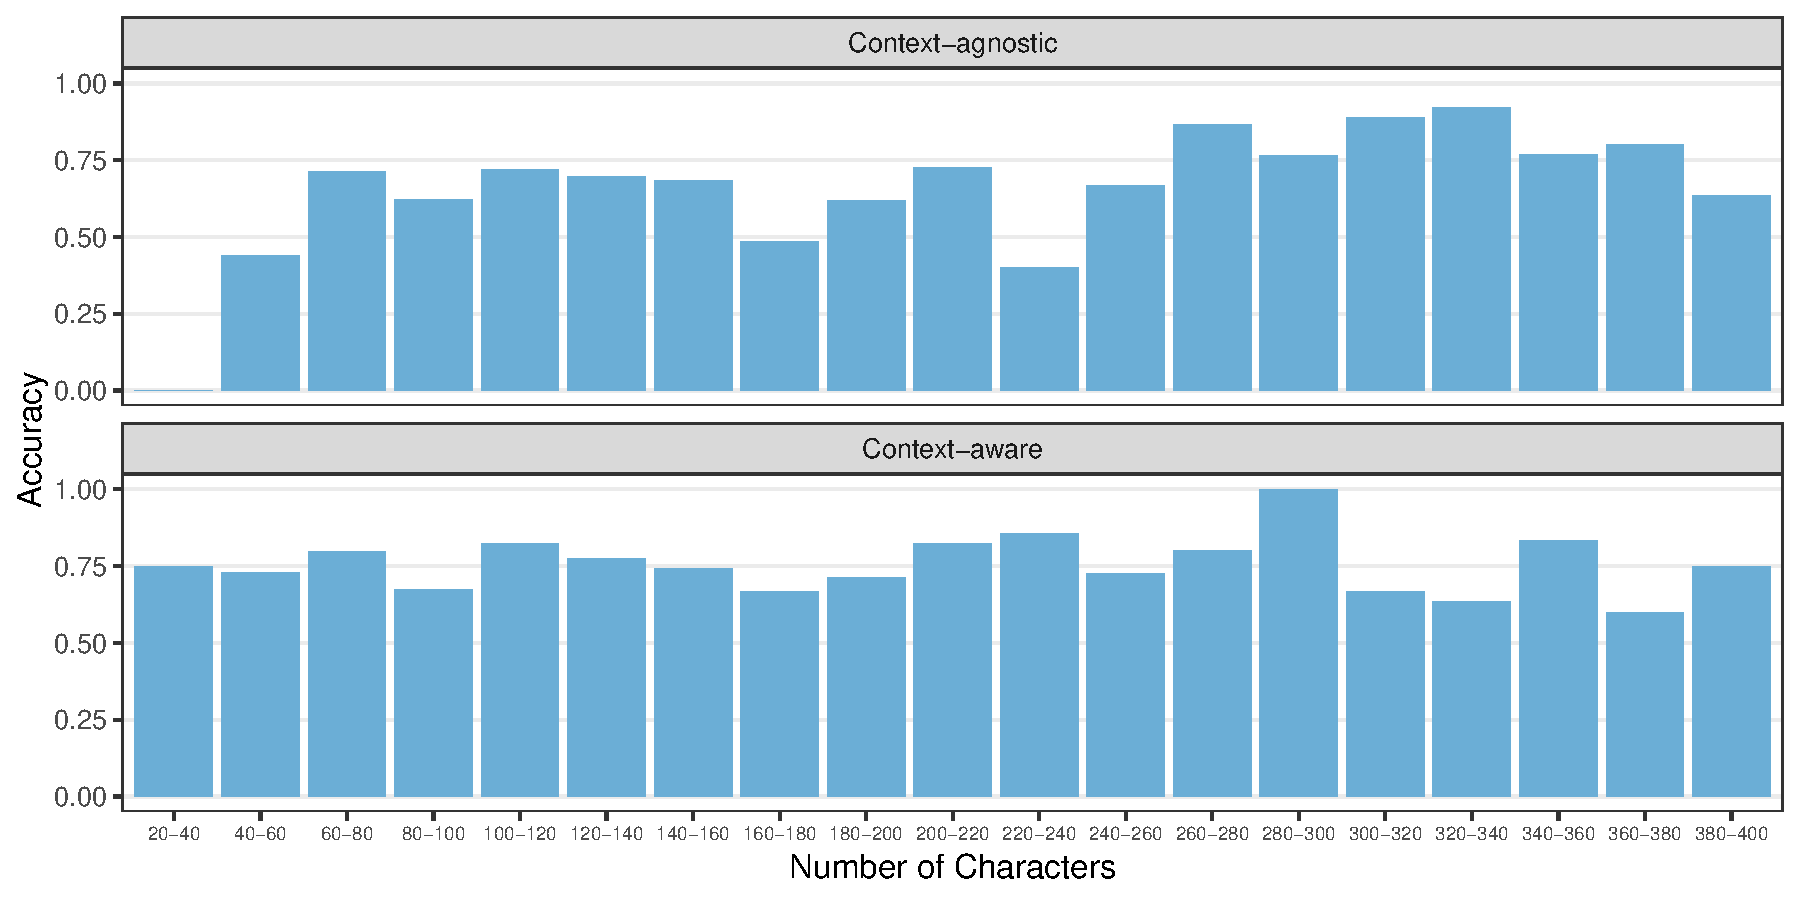
\includegraphics[width=1\textwidth]{graphs/experiments/length_acc.pdf}
  \end{center}
  \caption{A comparison of the performance between a conversation-agnostic model (only reply) with a conversation-aware model (PP, headline only root) in regard to length of comments.}
   \label{fig:exp_acc_len}
\end{figure}


\begin{figure}
  \begin{center}
    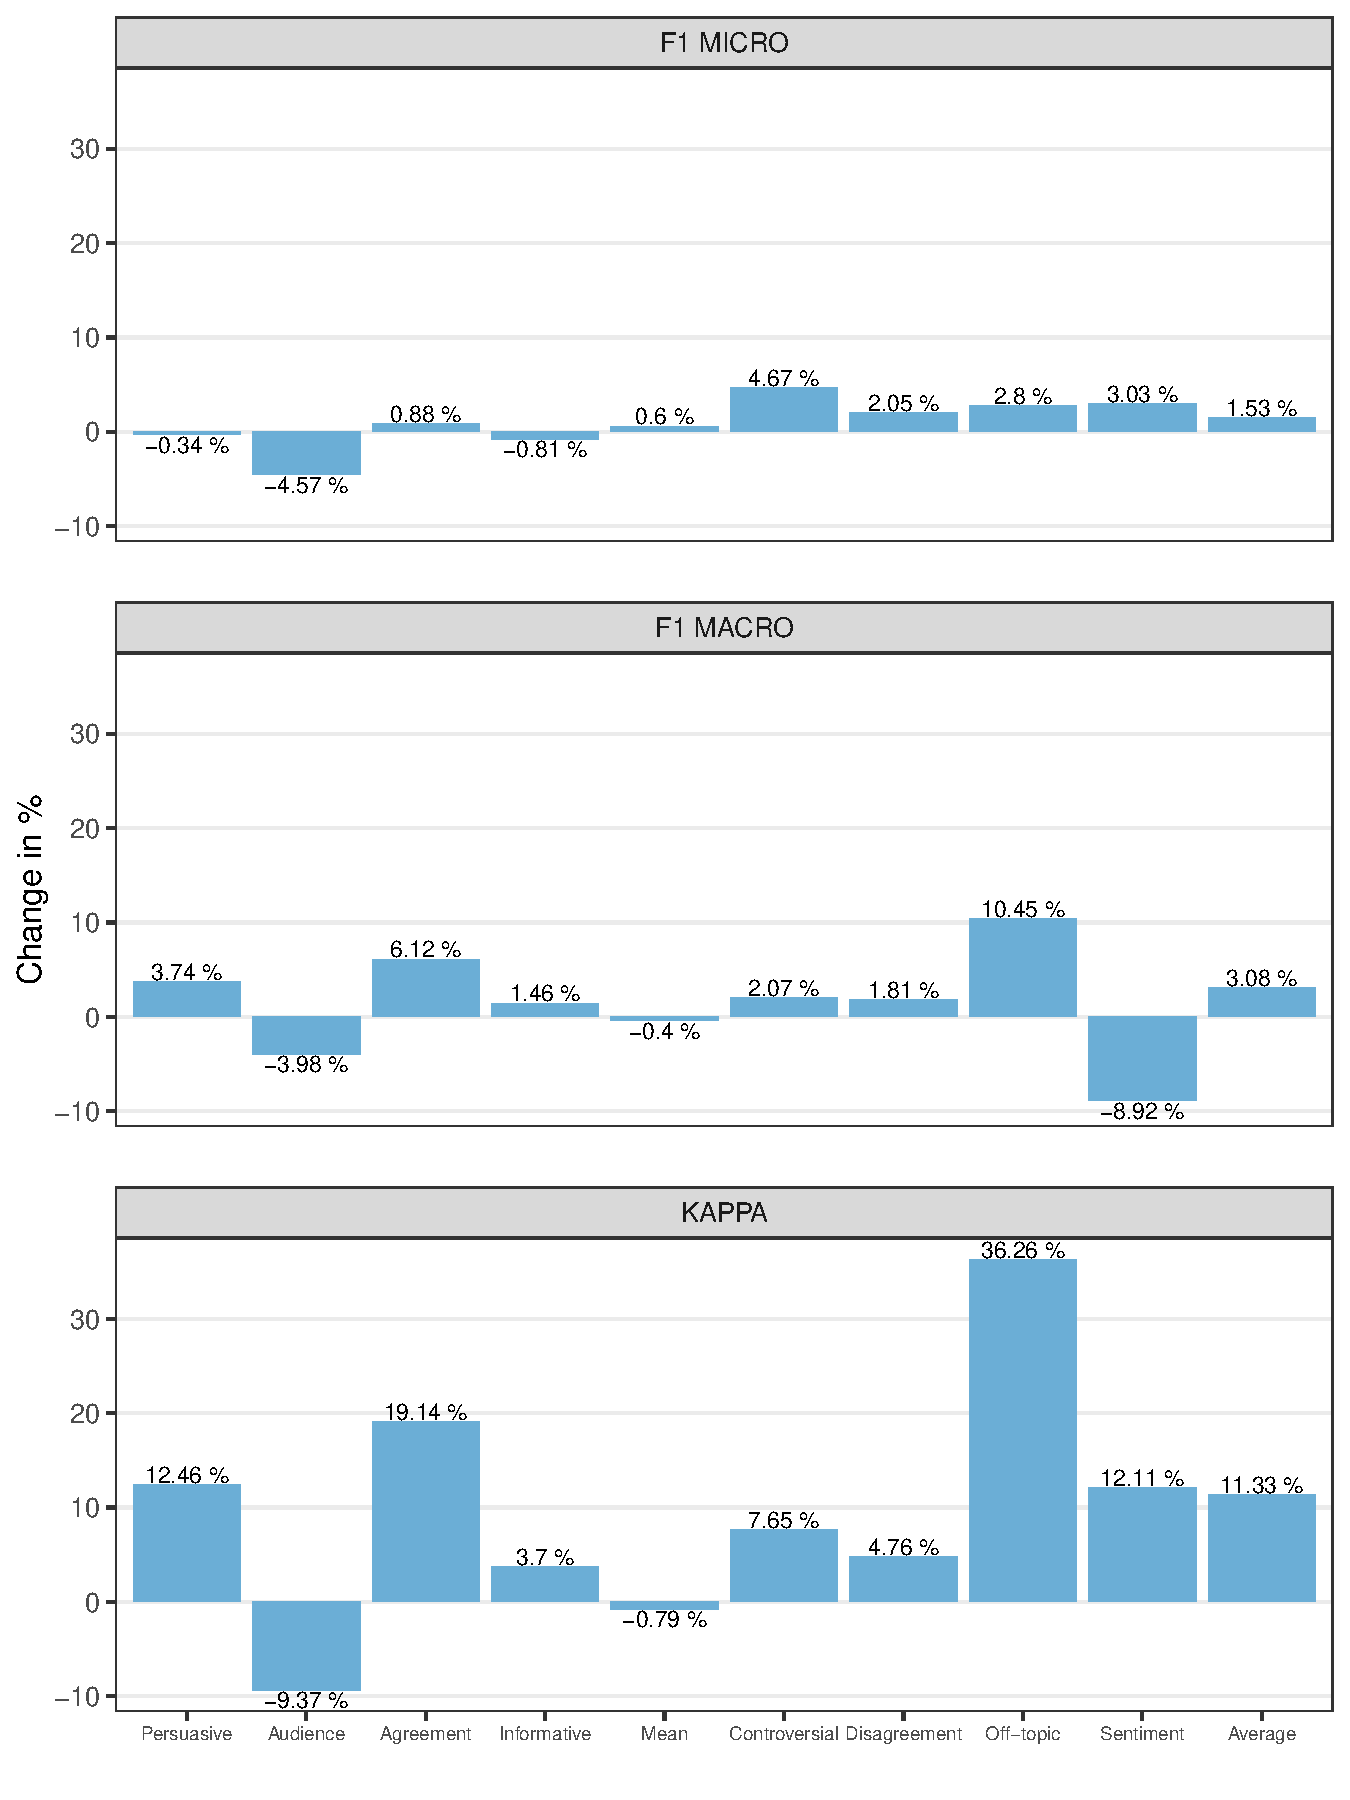
\includegraphics[width=1\textwidth]{graphs/experiments/changes.pdf}
  \end{center}
  \caption{The change in percent of the best conversation-agnostic model vs the best conversation-aware model based on Kappa.}
   \label{fig:res_changes}
\end{figure}

Finally, we speculate whether we have outperformed previously reported values.
Unfortunately, we cannot be sure how exactly the metrics were created.
The values were presented and also discussed in Section~\ref{subsec:ynacc_reported}.
The Kappa values that are presented come from this section.
We focus on Kappa to compare the performance of a model with a single metric.
There are multiple categories where the reported results are either impressive or poor:
Persuasive (0.79 or -0.173), Mean (0.693 or -0.238), Agreement (0.728 or -0.184), Off-topic (0.474 or -0.237).
For Audience, the values are so clear (0.816 or 0.575).
It is hard to make a definite statement about them.
However, for other categories we outperformed them clearly.
We can say for sure that we have outperformed YNACC for Controversial (0.158 or -0.024) and Disagreement (0.365 or 0.009).
The authors reveal in their publication that Informative (0.703 or -0.25) is below their ridge regression baseline.
So the value of 0.703 is impossible.
This means we have outperformed them clearly.
Also Sentiment with a reported F\textsubscript{1} of 0.43 is below our results of over 0.6 for the majority of approaches.
Since this is a four-class setup, the values ought to be averaged in some way.
We do not know how but we outperformed them in any way.


\subsection{Discussion}


The issue concerning the reported values makes it hard to compare our results.
However, we could demonstrate that we outperformed previous results in at  least three categories.
We were mainly reporting on the results on the validation set.
This has two reasons.
We want to set our work into perspective -- even this was only possible for three categories.
Moreover, the test values the dropped across all models considerably.
Generally, it is advised to report values on the test set, because it is likely that one has overfit parameters on the validation set.
So the validation results must be considered carefully.
However, our question was primarily whether it is essential to consider the conversational context is important.
And this can be answered by working on the validation as well as test results.
And the test sets contains further uncertainty, since they were annotated from a different group of people than the training and validation set.
Also the unnecessary noise of randomly assigning samples to classes, where  no majority wins is a problem.
So the drop in the models can be explained by the noise in the data as characteristics of the data.
In news comments, the words greatly differ from article to article.
More annotated data is needed to create better datasets to create more accurate results.

Our results allow to believe that the conversational context helped for certain categories.
It is not needed for all categories.
But for categories, that relate in some way to previous comments, the performance with context increased.
This allowed the model to get a deeper understanding of news comments.
To decide whether a comments agrees or disagrees, it helps to understand what was written before.
Also to decide whether a comment is off-topic, the previous comment help to make clear what the actual topic is.
That adding information about the article decreases the performance, may a problem of this approach.
Information about an article may duplicated immensely in the trainings sets.
So here Prepend Previous has some serious short-comings.
Further research is needed to overcome this.
Using separate sub-networks for the article and the comment may help.


\section{Experiments on One Million Posts Corpus}

In this section, we conduct two experiment on the dataset of German news which was described in Section~\ref{sec:ompc_ds}.

\subsection{Setup}

The conversation-agnostic model follows the same setup as already described in Section~\ref{ssssss:whaaatever} for experiments on YNACC.
A general German language model is required and it was presented in Section~\ref{sec:ulmfit_for_de}.
The language model is fine-tuned on the unlabeled comments until overfitting.
The OMPC datasets as well contains cross validation folds.
We re-use these to compare our results.
The model is trained for 100 epochs but stopped if the Kappa score did not improve for over 40 epochs.
The test value of the last epoch is used to determine a fold's performance.
The following parameters were used: a dropout multiplier of 0.8, a learning rate of 0.001, and a batch size of 128.

For the conversation-aware model, the comments were preprocessed with Prepend Previous.
Since the comments were originally created in a tree-like discussion structure, the Prepend Previous differs from YNACC.
It can happen that an intermediate-comment can have more than one child.
Thus this comment appears multiple times in the samples.
To avoid duplicates of those comments, all comment chains are truncated to 400 tokens.
This should ensure that the number of duplications is low.
Since classes are unbalanced, the loss was weighted according to the distribution of classes in the appropriate fold.

\subsection{Results}
\label{sec:ompc_results}

The results are presented in Table~\ref{tab:res3}.
We follow the metrics of related literature and show the Precision, Recall and F\textsubscript{1} in regard to the minority class.
The conversation-aware model achieved lower results than a conversation-agnostic model in all categories.
However, the context-agnostic model outperformed previously reported results besides for the categories Feedback and Off-topic.
There does not exists a previously reported result for Neutral.
H{\"a}ring et al.~\cite{haring2018addressed} only reported results for Feedback.
The best value of all of the experiments by Schabus et al.~\cite{schabus_academic-industrial_nodate} are chosen as reference.
The F\textsubscript{1} increased for Positive and Inappropriate by 79.3\% and 25.1\%, respectively.

\begin{table}
\caption{The cross-validation results on OMPC. The best models by Schabus et al.~\cite{schabus_academic-industrial_nodate}, based on their F\textsubscript{1} score, are chosen as reference. H{\"a}ring~et al.\cite{haring2018addressed} only report results for Feedback. Only the F\textsubscript{1} score is highlighted}
\begin{tabular}{ l l l l l l}
\toprule
Category & Metric & Schabus~\cite{schabus_academic-industrial_nodate} & H{\"a}ring~\cite{haring2018addressed} & Context-agnostic & Context-aware\\
\midrule
\addlinespace[2ex]
\multirow{3}{*}{Negative} & Precision & 0.6112 & & 0.6044 & 0.5802 \\
& Recall & 0.6014 & & 0.6168 & 0.5311 \\
& F\textsubscript{1} & 0.6063 & & \textbf{0.6089} & 0.5290 \\ \addlinespace[2ex]
\multirow{3}{*}{Neutral} & Precision & & & 0.6124 & 0.5478 \\
& Recall & & & 0.6155 & 0.5305 \\
& F\textsubscript{1} & &  & \textbf{0.6073} & 0.5089 \\ \addlinespace[2ex]
\multirow{3}{*}{Positive} & Precision & 0.1020 & & 0.4850 & 0.3299 \\
& Recall & 0.3488 & & 0.2422 & 0.1797 \\
& F\textsubscript{1} & 0.1579 & & \textbf{0.2831} & 0.1418 \\ \addlinespace[2ex]
\multirow{3}{*}{Off-topic} & Precision & 0.2472 & & 0.4637 & 0.4344 \\
& Recall & 0.6086 & & 0.2771 & 0.2169 \\
& F\textsubscript{1} & \textbf{0.3516} & & 0.3431 & 0.2603 \\ \addlinespace[2ex]
\multirow{3}{*}{Inappr} & Precision & 0.1340 & & 0.4585 & 0.4531 \\
& Recall & 0.5776 & & 0.2010 & 0.1358 \\
& F\textsubscript{1} & 0.2175 & & \textbf{0.2720} & 0.1939 \\ \addlinespace[2ex]
\multirow{3}{*}{Discrim} & Precision & 0.1207 & & 0.3288 & 0.4881 \\
& Recall & 0.5922 & & 0.1512 & 0.1080 \\
& F\textsubscript{1} & 0.2005 & & \textbf{0.2037} & 0.1596 \\ \addlinespace[2ex]
\multirow{3}{*}{Feedback} & Precision & 0.5311 & 0.85 & 0.8178 & 0.8424 \\
& Recall & 0.7356 & 0.83 & 0.6383 & 0.5362 \\
& F\textsubscript{1} & 0.6168 & \textbf{0.84} & 0.7099 & 0.6443 \\ \addlinespace[2ex]
\multirow{3}{*}{Personal} & Precision & 0.6247 & & 0.8787 & 0.7329 \\
& Recall & 0.8123 & & 0.6271 & 0.6516 \\
& F\textsubscript{1} & 0.7063 & & \textbf{0.7188} & 0.6670 \\ \addlinespace[2ex]
\multirow{3}{*}{Argument} & Precision & 0.5457 & & 0.7612 & 0.6854 \\
& Recall & 0.7652 & & 0.5644 & 0.5592 \\
& F\textsubscript{1} & 0.6371 & & \textbf{0.6430} & 0.6026 \\ \addlinespace[2ex]
\bottomrule
\end{tabular}
\label{tab:res3}
\end{table}

\subsection{Discussion}

Further research is needed to evaluate whether the conversational context improves the performance for the OMPC datasets.
The current results for context-aware models are far below conversation-agnostic models.
This may have various reasons.
The amount of annotated is low and especially the number of test samples with for the most categories of about 300 is low.
This leads to fluctuating performances across the folds.
Different variations of early stopping should be explored.
Setting the same parameters for all folds may not have been the best decision.
For some folds, the model needs to get more carefully trained with more regularization.
In other folds, the model did not converge at all.
To tune hyper-parameters, the training folds should be split into an addition validation fold.
Then, the parameters need to get tuned on the validation set before measuring the final performance on the test set.
Nevertheless, the conversation-agnostic model outperformed the featured-based models by Schabus in almost all cases.
Even though there is, i.e., no information about the casing in the text.
The casing in news comments bears information.
So for the future, a German language model with casing should be trained.

